\documentclass[aspectratio=169]{beamer}
\usepackage{will_handley_beamer}
\usepackage{title_page}
\usetikzlibrary{arrows,arrows.meta,automata,positioning}

% Commands
% --------
% - \arxiv{arxiv number}
% - \cols{width}{lh column}{rh column}
% -  \begin{fig(left|right)}[fractional width (e.g 0.6) ]{name of image}
%        content of other column
%    \end{fig(left|right)}

% Talk details
% ------------
\title{\texttt{PolySwyft}}
\subtitle{a sequential simulation-based nested sampler}
\date{16\textsuperscript{th} May 2024}

\begin{document}

\begin{frame}
    \titlepage
\end{frame}

\begin{frame}
    \frametitle{Contents}
    \begin{columns}
        \column{0.77\textwidth}
        \begin{enumerate}
            \item Likelihood- vs Simulation-based inference (LBI vs SBI) 
            \item Neural Ratio estimation (NRE)
            \item Nested sampling (NS)
            \item NS+NRE
            \item Future prospects
        \end{enumerate}
        Stems from over a year of discussion, with the majority of the work done by Kilian Scheutwinkel (PhD student).
        \column{0.23\textwidth}
        \begin{overpic}[width=\textwidth]{figures/students/kilian_scheutwinkel.jpg}
            \put(5,5) {\textcolor{white}{Kilian Scheutwinkel}}
        \end{overpic}
        \begin{overpic}[width=\textwidth]{figures/students/christoph_weniger.jpg}
            \put(10,5) {\textcolor{white}{Christoph Weniger}}
        \end{overpic}
    \end{columns}
\end{frame}

\begin{frame}
    \frametitle{LBI: Likelihood-based inference}
    \begin{columns}
        \column{0.5\textwidth}
        The standard approach if you are fortunate enough to have a likelihood function $\only<1-2>{P(D|\theta)}\only<3->{\C[2]{\mathcal{L}(D|\theta)}}$: 
        \[
            \only<1-2>{
                P(\theta|D) = \frac{P(D|\theta)P(\theta)}{P(D)}
            }
            \only<2>{
                \qquad
                \C[0]{\text{Posterior}} = \frac{\C[2]{\text{Likelihood}}\times\C[1]{\text{Prior}}}{\C[3]{\text{Evidence}}}
            }
            \only<3>{
                \C[0]{\mathcal{P}(\theta|D)} = \frac{\C[2]{\mathcal{L}(D|\theta)}\C[1]{\pi(\theta)}}{\C[3]{\mathcal{Z}(D)}}
                \qquad
                \C[0]{\text{Posterior}} = \frac{\C[2]{\text{Likelihood}}\times\C[1]{\text{Prior}}}{\C[3]{\text{Evidence}}}
            }
            \only<4>{
                P(\theta|D) P(D) = P(\theta,D) = P(D|\theta)P(\theta), \qquad
            }
            \only<5>{
                \C[0]{\mathcal{P}}\times\C[3]{\mathcal{Z}} = \C[4]{\mathcal{J}} = \C[2]{\mathcal{L}}\times\C[1]{\pi}, \qquad \C[4]{\text{Joint}} = \C[4]{\mathcal{J}} = P(\theta,D)
            }
        \]
        \vspace{-10pt}
        \begin{enumerate}
            \item Define \C[1]{prior $\pi(\theta)$} 
                \begin{itemize}
                    \item spend some time being philosophical
                \end{itemize}
            \item Sample \C[0]{posterior $\mathcal{P}(\theta|D)$} 
                \begin{itemize}
                    \item use out-of-the-box MCMC tools such as\\ \texttt{emcee} or \texttt{MultiNest}
                    \item make some triangle plots
                \end{itemize}
            \item Optionally compute \C[3]{evidence $\mathcal{Z}(D)$}
                \begin{itemize}
                    \item e.g. nested sampling or parallel tempering
                    \item do some model comparison (i.e. science)
                    \item talk about tensions
                \end{itemize}
        \end{enumerate}
        \column{0.5\textwidth}
        \hfill%
        \begin{overpic}[width=0.6\textwidth]{figures/des_parameters.pdf}
            \put(-40,90) {DES Y5 SN Ia}
            \put(-40,80) {\arxiv{2401.02929}}
        \end{overpic}
        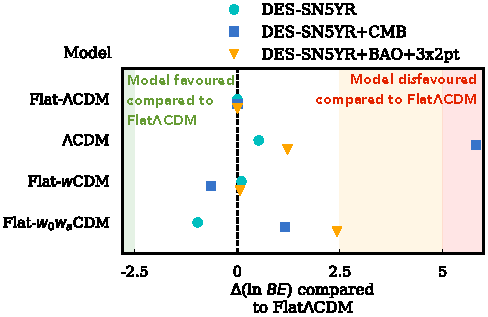
\includegraphics[width=0.5\textwidth]{figures/des_model_comparison.pdf}%
        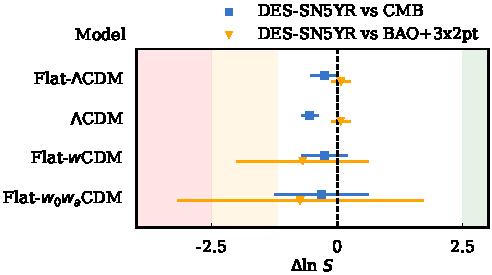
\includegraphics[width=0.5\textwidth]{figures/des_suspiciousness.pdf}
    \end{columns}
\end{frame}

\begin{frame}
    \frametitle{SBI: Simulation-based inference}
    \begin{columns}
        \column{0.5\textwidth}
        \begin{itemize}
            \item What do you do if you don't know \C[2]{$\mathcal{L}(D|\theta)$}?
            \item If you have a simulator/forward model $\theta \rightarrow D$
                defines an \C[2]{\emph{implicit} likelihood~$\mathcal{L}$}.
            \item Simulator generates samples from $\C[2]{\mathcal{L}(\cdot|\theta)}$.
            \item With a prior $\C[1]{\pi}(\theta)$ can generate samples from \C[4]{joint distribution}~$\C[4]{\mathcal{J}(\theta,D)}=\C[2]{\mathcal{L}(D|\theta)}\C[1]{\pi(\theta)}$\\\hfill \emph{the ``probability of everything''}.
            \item Task of SBI is take joint~$\C[4]{\mathcal{J}}$ samples and learn \C[0]{posterior $\mathcal{P}(\theta|D)$} and \C[3]{evidence $\mathcal{Z}(D)$} \\\hfill and possibly \C[2]{likelihood $\mathcal{L}(D|\theta)$}.
            \item Present state of the art achieves this using \emph{machine learning} (neural networks).
                \begin{itemize}
                    \item My group's research tries to removes machine learning \tthref{github.com/handley-lab/lsbi}.

                \end{itemize}
            %\item Present SotA: NPE, NLE, NJE, NRE
            %\item SBI \& forward modelling force us to think about data space~$D$ \& parameter space~$\theta$.
        \end{itemize}
        \column{0.5\textwidth}
        \includegraphics<1>[page=1, width=\textwidth]{figures/sbi_parameter_estimation.pdf}%
        \includegraphics<2>[page=2, width=\textwidth]{figures/sbi_parameter_estimation.pdf}%
        \includegraphics<3>[page=3, width=\textwidth]{figures/sbi_parameter_estimation.pdf}%
        \includegraphics<4>[page=4, width=\textwidth]{figures/sbi_parameter_estimation.pdf}%
        \includegraphics<5>[page=5, width=\textwidth]{figures/sbi_parameter_estimation.pdf}%
        \includegraphics<6>[page=6, width=\textwidth]{figures/sbi_parameter_estimation.pdf}%
        \includegraphics<7>[page=7, width=\textwidth]{figures/sbi_parameter_estimation.pdf}%
        \includegraphics<8>[page=8, width=\textwidth]{figures/sbi_parameter_estimation.pdf}%
        \includegraphics<9>[page=9, width=\textwidth]{figures/sbi_parameter_estimation.pdf}%
        \includegraphics<10>[page=10, width=\textwidth]{figures/sbi_parameter_estimation.pdf}%
        \includegraphics<11>[page=11, width=\textwidth]{figures/sbi_parameter_estimation.pdf}%
        \includegraphics<12>[page=12, width=\textwidth]{figures/sbi_parameter_estimation.pdf}%
        \includegraphics<13>[page=13, width=\textwidth]{figures/sbi_parameter_estimation.pdf}%
        \includegraphics<14>[page=14, width=\textwidth]{figures/sbi_parameter_estimation.pdf}%
        \includegraphics<15>[page=15, width=\textwidth]{figures/sbi_parameter_estimation.pdf}%
        \includegraphics<16>[page=16, width=\textwidth]{figures/sbi_parameter_estimation.pdf}%
        \includegraphics<17>[page=17, width=\textwidth]{figures/sbi_parameter_estimation.pdf}%
        \includegraphics<18>[page=18, width=\textwidth]{figures/sbi_parameter_estimation.pdf}%
        \includegraphics<19>[page=19, width=\textwidth]{figures/sbi_parameter_estimation.pdf}%
        \includegraphics<20>[page=20, width=\textwidth]{figures/sbi_parameter_estimation.pdf}%
        \includegraphics<21>[page=21, width=\textwidth]{figures/sbi_parameter_estimation.pdf}%
    \end{columns}
\end{frame}

\begin{frame}
    \frametitle{Why SBI?}
    \begin{columns}
        \column{0.6\textwidth}
        SBI is useful because:
        \begin{enumerate}
            \item If you don't have a likelihood, you can still do inference
                \begin{itemize}
                    \item This is the usual case beyond CMB cosmology
                \end{itemize}
            \item Faster than LBI
                \begin{itemize}
                    \item emulation -- also applies to LBI in principle
                \end{itemize}
            \item No need to pragmatically encode fiducial cosmologies
                \begin{itemize}
                    \item Covariance computation implicitly encoded in simulations
                    \item Highly relevant for disentangling tensions \& systematics
                \end{itemize}
            \item Equips AI/ML with Bayesian interpretability
            \item Lower barrier to entry than LBI
                \begin{itemize}
                    \item Much easier to forward model a systematic
                    \item Emerging set of plug-and-play packages
                    \item For this reason alone, it will come to dominate scientific inference
                \end{itemize}
        \end{enumerate}
        \column{0.4\textwidth}
        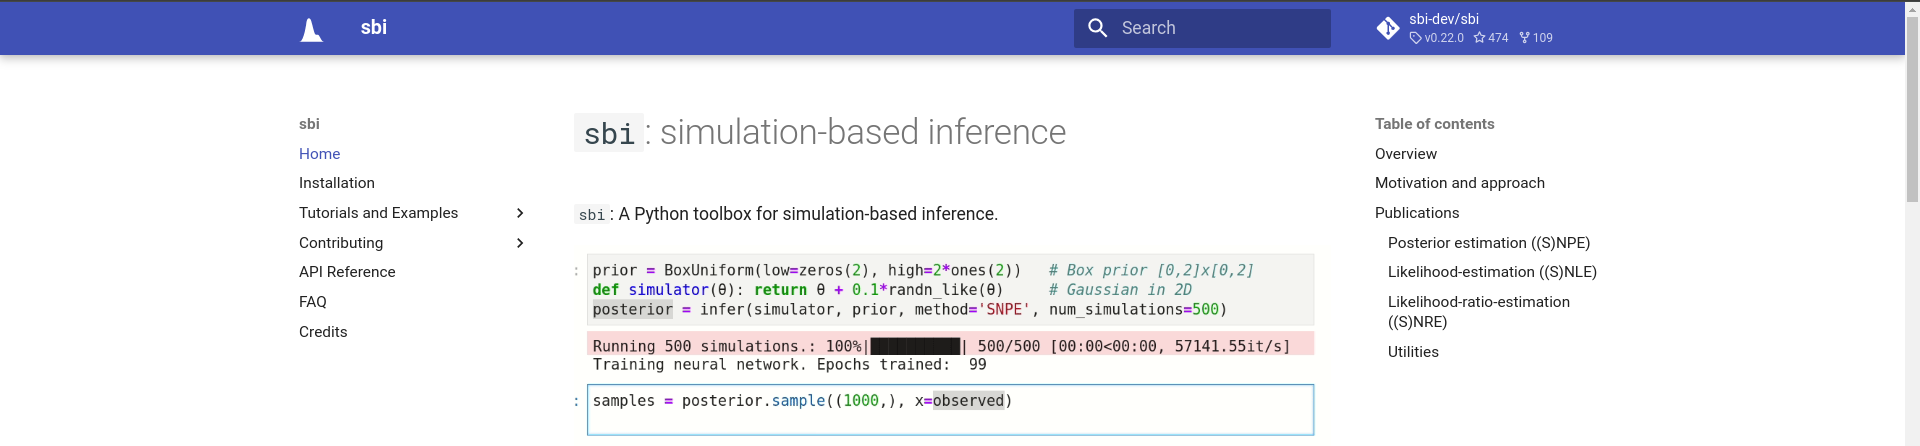
\includegraphics[width=\textwidth]{figures/sbi_screenshot}
        \href{https://github.com/sbi-dev}{github.com/sbi-dev}
        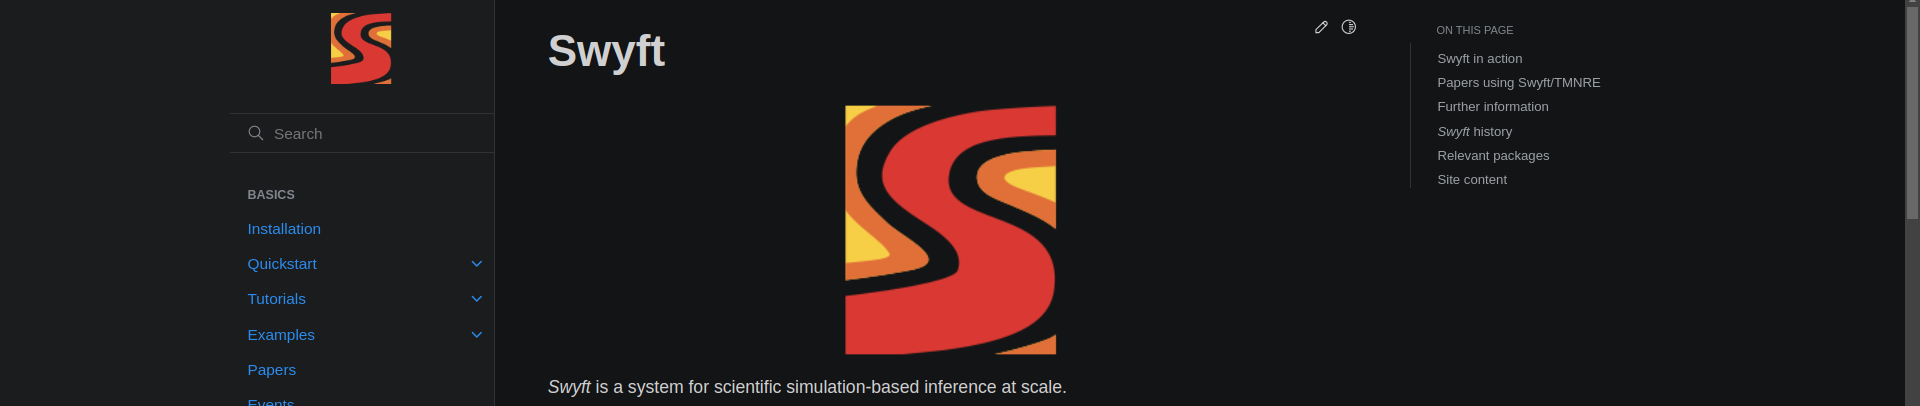
\includegraphics[width=\textwidth]{figures/swyft_screenshot}
        \href{https://github.com/undark-lab/swyft}{github.com/undark-lab/swyft}
        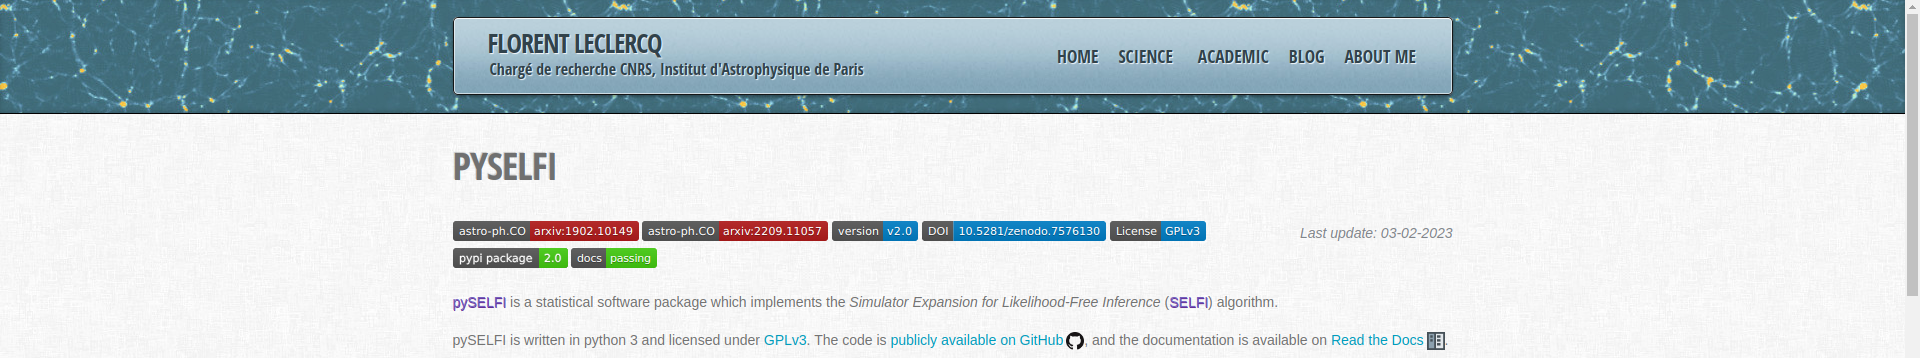
\includegraphics[width=\textwidth]{figures/selfi_screenshot}
        \href{https://github.com/florent-leclercq/pyselfi}{github.com/florent-leclercq/pyselfi}
        
\includegraphics[width=\textwidth]{figures/delfi_screenshot}
        \href{https://github.com/justinalsing/pydelfi}{github.com/justinalsing/pydelfi}
    \end{columns}
\end{frame}

\begin{frame}
    \frametitle{Why aren't we currently using SBI in cosmology?}
    \begin{columns}
        \column{0.4\textwidth}
        \begin{itemize}
            \item Short answer: we are!
                \begin{itemize}
                    \item Mostly for weak lensing
                    \item 2024 has been the year it has started to be applied to real data.
                \end{itemize}
            \item Longer answer: SBI requires mock data generation code
            \item Most data analysis codes were built before the generative paradigm.
            \item It's still a lot of work to upgrade cosmological likelihoods  to be able to do this (e.g.\ \texttt{plik} \& \texttt{camspec}).
        \end{itemize}
        \column{0.3\textwidth}
        
\includegraphics[width=\textwidth]{figures/sbi_papers/clusters.pdf}
        \vspace{10pt}\\
        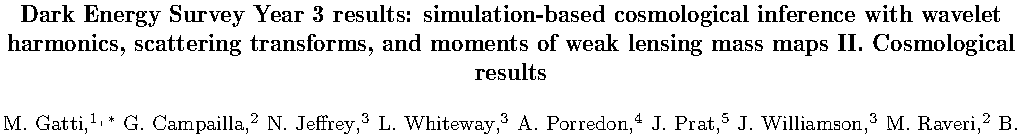
\includegraphics[width=\textwidth]{figures/sbi_papers/des.pdf}
        \vspace{10pt}\\
        
\includegraphics[width=\textwidth]{figures/sbi_papers/gw.pdf}
        \vspace{10pt}\\
        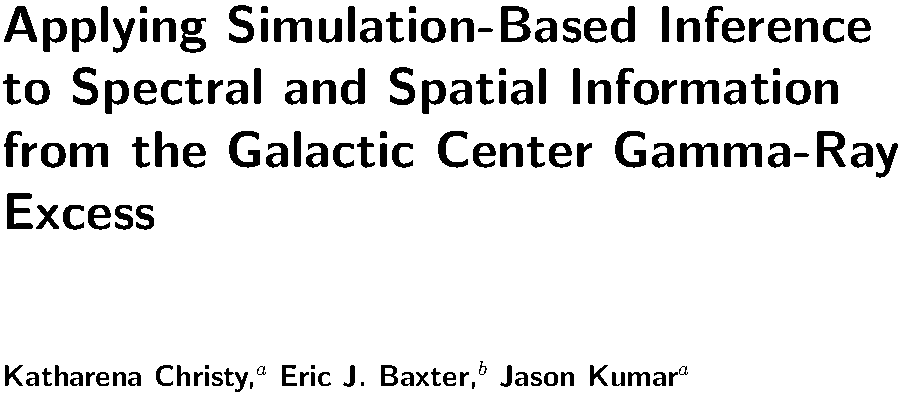
\includegraphics[width=\textwidth]{figures/sbi_papers/center.pdf}
        \column{0.3\textwidth}
        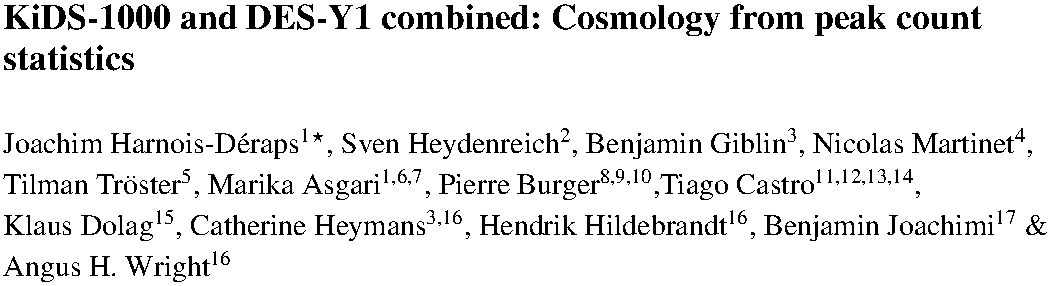
\includegraphics[width=\textwidth]{figures/sbi_papers/kidsdes.pdf}
        \vspace{10pt}\\
        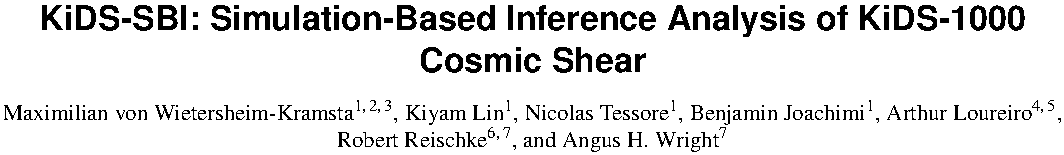
\includegraphics[width=\textwidth]{figures/sbi_papers/kids.pdf}
        \vspace{10pt}\\
        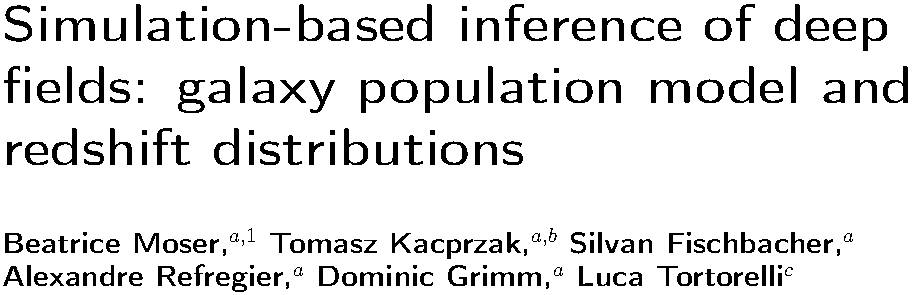
\includegraphics[width=\textwidth]{figures/sbi_papers/population.pdf}
        \vspace{10pt}\\
        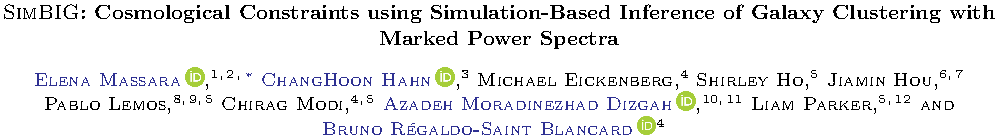
\includegraphics[width=\textwidth]{figures/sbi_papers/simbig.pdf}
    \end{columns}
\end{frame}

\begin{frame}
    \frametitle{Neural Ratio Estimation}
    \begin{columns}
        \column{0.5\textwidth}
        \begin{itemize}
            \item SBI flavours: {\small \hfill\tthref{github.com/sbi-dev/sbi}}
                {\small
                    \begin{description}
                        \item[NPE] Neural posterior estimation
                        \item[NLE] Neural likelihood estimation
                        \item[NJE] Neural joint estimation
                        \item[NRE] Neural ratio estimation
                    \end{description}
                }
            \item NRE recap:
                \begin{enumerate}
                    \item Generate joint samples $(\theta,D)\sim\C[4]{\mathcal{J}}$
                        \label{step:joint}
                        \begin{itemize}
                            \item \textit{straightforward if you have a simulator:\\ $\theta\sim\C[1]{\pi(\cdot)}$, $D\sim\C[2]{\mathcal{L}(\cdot|\theta)}$}
                        \end{itemize}
                    \item Generate separated samples $\theta\sim\C[1]{\pi}$, $D\sim\C[3]{\mathcal{Z}}$\label{step:sep}
                        \begin{itemize}
                            \item \textit{aside: can shortcut step~\ref{step:sep} by scrambling the $(\theta,D)$ pairings from step~\ref{step:joint}}
                        \end{itemize}
                    \item Train probabilistic classifier $p$ to distinguish whether $(\theta,D)$ came from $\C[4]{\mathcal{J}}$ or $\C[1]{\pi}\times\C[3]{\mathcal{Z}}$.
                    \item $\frac{p}{1-p} = \C[5]{r} = \frac{P(\theta,D)}{P(\theta)P(D)} 
                        =
                        \frac{\C[4]{\mathcal{J}}}{\C[1]{\pi}\times\C[3]{\mathcal{Z}}} = \frac{\C[2]{\mathcal{L}}}{\C[3]{\mathcal{Z}}} = \frac{\C[0]{\mathcal{P}}}{\C[1]{\pi}}$.
                    \item Use ratio $\C[5]{r}$ for parameter estimation $\C[0]{\mathcal{P}} = \C[5]{r}\C[1]\times {\pi}$
                \end{enumerate}
        \end{itemize}
        \column{0.5\textwidth}
        \only<1|handout:0>{
            \begin{tikzpicture}[node distance=1cm, every neuron/.style={circle, draw, minimum size=1cm},]
                \node[every neuron/.try] (j2)  {};
                \node[every neuron/.try, above left = 0cm and 0.5cm of j2] (theta) { $\theta$};
                \node[every neuron/.try, below left = 0cm and 0.5cm of j2] (D) { $D$};
                \node[every neuron/.try, above = 0.5cm of j2] (j1) {};
                \node[every neuron/.try, below = 0.5cm of j2] (j3) {};
                \node[every neuron/.try, above right = 0cm and 0.5cm of j2] (h1) {};
                \node[every neuron/.try, below right = 0cm and 0.5cm of j2] (h2) {};
                \node[every neuron/.try, right = 1.3cm of j2] (p) { $p$};
                \node[every neuron/.try, right = 0.5cm of p] (logr) { $\C[5]{r}$};
                \draw[-] (theta) -- (j1);
                \draw[-] (D) -- (j1);
                \draw[-] (theta) -- (j2);
                \draw[-] (D) -- (j2);
                \draw[-] (theta) -- (j3);
                \draw[-] (D) -- (j3);
                \draw[-] (j1) -- (h1);
                \draw[-] (j1) -- (h2);
                \draw[-] (j2) -- (h1);
                \draw[-] (j2) -- (h2);
                \draw[-] (j3) -- (h1);
                \draw[-] (j3) -- (h2);
                \draw[-] (h1) -- (p);
                \draw[-] (h2) -- (p);
                \draw[-] (p) -- (logr);
                \node[below =0.5cm of logr] {\includegraphics[page=22, width=0.5\textwidth]{figures/sbi_parameter_estimation.pdf}};
            \end{tikzpicture}
        }
        \only<2>{
            \begin{exampleblock}{Bayesian proof}
                \begin{itemize}
                    \item Let $M_{\C[4]{\mathcal{J}}}$: $(\theta,D)\sim\C[4]{\mathcal{J}}$, $M_{\C[1]{\pi}\C[3]{\mathcal{Z}}}$: $(\theta,D)\sim\C[1]{\pi}\times\C[3]{\mathcal{Z}}$
                    \item Classifier gives
                        ${p(\theta,D) = P(M_{\C[4]{\mathcal{J}}}|\theta,D) = 1- P(M_{\C[1]{\pi}\C[3]{\mathcal{Z}}}|\theta,D)}$
                    \item Bayes theorem then shows
                        ${\frac{p}{1-p}=\frac{P(M_{\C[4]{\mathcal{J}}}|\theta,D)}{P(M_{\C[1]{\pi}\C[3]{\mathcal{Z}}}|\theta,D)} = \frac{P(\theta,D|M_{\C[4]{\mathcal{J}}})P(M_{\C[4]{\mathcal{J}}})}{P(\theta,D|M_{\C[1]{\pi}\C[3]{\mathcal{Z}}})P(M_{\C[1]{\pi}\C[3]{\mathcal{Z}}})} = 
                        \frac{\C[4]{\mathcal{J}}}{\C[1]{\pi}\C[3]{\mathcal{Z}}}}$, \\
                        where we have assumed 
                        \begin{itemize}
                            \item $P(M_{\C[4]{\mathcal{J}}}) = P(M_{\C[1]{\pi}\C[3]{\mathcal{Z}}})$,
                        \end{itemize}
                        and by definition
                        \begin{itemize}
                            \item $\C[4]{\mathcal{J}(\theta,D)} = P(\theta,D|M_{\C[4]{\mathcal{J}}})$
                            \item $\C[1]{\pi(\theta)}\C[3]{\mathcal{Z}(D)} = P(\theta,D|M_{\C[1]{\pi}\C[3]{\mathcal{Z}}})$.
                        \end{itemize}
                \end{itemize}
            \end{exampleblock}
        }
        \only<3|handout:0>{
            \begin{block}{Why I like NRE}
                \begin{itemize}
                    \item The link between classification and inference is profound.
                    \item Density estimation is hard -- Dimensionless $r$ divides out the hard-to-calculate parts.
                \end{itemize}
            \end{block}
            \begin{block}{Why I don't like NRE}
                \begin{itemize}
                    \item Practical implementations require marginalisation~\arxiv{2107.01214}, or autoregression~\arxiv{2308.08597}.
                    \item Model comparison and parameter estimation are separate~\arxiv{2305.11241}.
                \end{itemize}
            \end{block}
        }
    \end{columns}
\end{frame}

\begin{frame}
    \frametitle{TMNRE: Truncated Marginal Neural Ratio Estimation}
    \framesubtitle{\texttt{swyft}: \tthref{github.com/undark-lab/swyft}}
    \begin{columns}
        \column{0.55\textwidth}
        \begin{itemize}
            \item Two tricks for practical NRE:
        \end{itemize}
        \begin{block}{Marginalisation}
            \begin{itemize}
                \item Only consider one or two parameters at a time.
                \item Fine if your goal is to produce triangle plots.
                \item Problematic if information is contained jointly in more than two parameters.
            \end{itemize}
        \end{block}
        \begin{block}{Truncation}
            \begin{itemize}
                \item focus parameters $\theta$ on a subset of the prior which reproduces observed data $D_\text{obs}$
                \item region is somewhat arbitrary (usually a box)
                \item not amortised, sounds a bit like ABC
            \end{itemize}
        \end{block}
        \column{0.45\textwidth}
        \begin{overpic}[width=\textwidth]{figures/tmnre}
            \put(70,0) {\arxiv{2111.08030}}
        \end{overpic}
    \end{columns}
\end{frame}

\begin{frame}
    \frametitle{Nested sampling: numerical Lebesgue integration}
    \begin{columns}
        \column{0.5\textwidth}
        \fbox{\parbox{\textwidth}{
                \begin{itemize}
                    \item[0.] Start with $N$ random samples over the space.
                    \item[i.] Delete outermost sample, and replace with a new random one at higher integrand value.
        \end{itemize}}}
        \vspace{-5pt}
        \begin{itemize}
            \item The ``live points'' steadily contract around the peak(s) of the function.
            \item Discarded ``dead points'' can be weighted to form posterior, prior, or anything in between.
            \item Estimates the \textbf{density of states} and calculates evidences \& partition functions.
            \item The evolving ensemble of live points allows:
                \begin{itemize}
                    \item implementations to self-tune,
                    \item exploration of multimodal functions,
                    \item global and local optimisation.
                \end{itemize}
        \end{itemize}
        \column{0.5\textwidth}
        \includegraphics<1|handout:0>[width=\textwidth,page=1]{figures/himmelblau}%
        \includegraphics<2|handout:0>[width=\textwidth,page=2]{figures/himmelblau}%
        \includegraphics<3|handout:0>[width=\textwidth,page=3]{figures/himmelblau}%
        \includegraphics<4|handout:0>[width=\textwidth,page=4]{figures/himmelblau}%
        \includegraphics<5|handout:0>[width=\textwidth,page=5]{figures/himmelblau}%
        \includegraphics<6|handout:0>[width=\textwidth,page=6]{figures/himmelblau}%
        \includegraphics<7|handout:0>[width=\textwidth,page=7]{figures/himmelblau}%
        \includegraphics<8|handout:0>[width=\textwidth,page=14]{figures/himmelblau}%
        \includegraphics<9->[width=\textwidth,page=15]{figures/himmelblau}%
    \end{columns}
\end{frame}

\begin{frame}
    \frametitle{Implementations of Nested Sampling \arxiv{2205.15570}(NatReview)}
    \begin{columns}[t]
        \column{0.3\textwidth}
        \texttt{MultiNest}~\arxiv{0809.3437}
        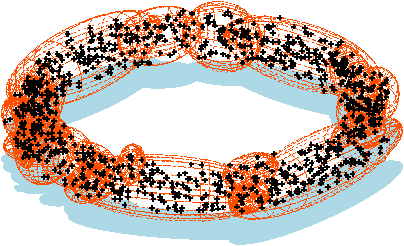
\includegraphics[width=\textwidth]{figures/multinest}
        \texttt{UltraNest}~\arxiv{2101.09604}
        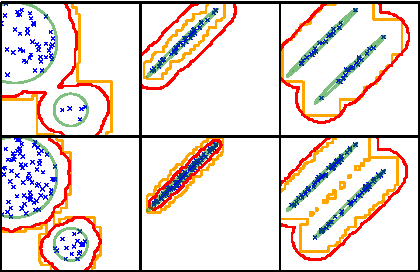
\includegraphics[width=\textwidth]{figures/radfriends}
        \texttt{nautilus}~\arxiv{2306.16923} 
        \column{0.4\textwidth}
        \texttt{PolyChord}~\arxiv{1506.00171}
        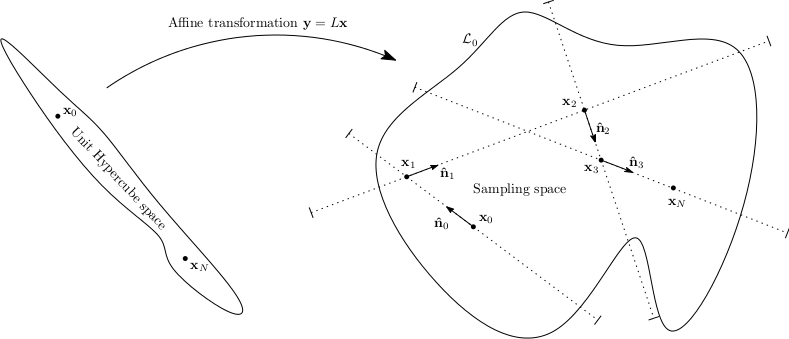
\includegraphics[width=\textwidth]{figures/polychord}
        \vfill
        \texttt{NeuralNest}~\arxiv{1903.10860}
        \begin{columns}
            \column{0.55\textwidth}
            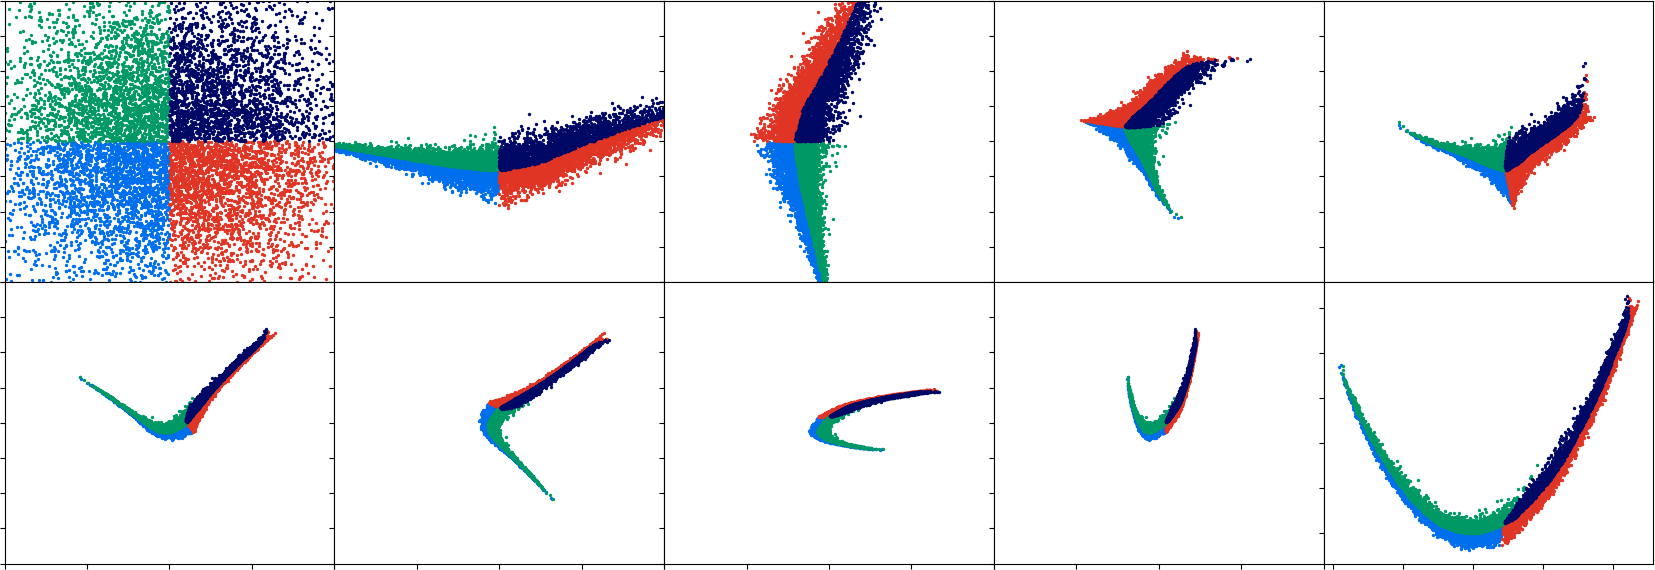
\includegraphics[width=\textwidth]{figures/rosenbrock_flow.png}
            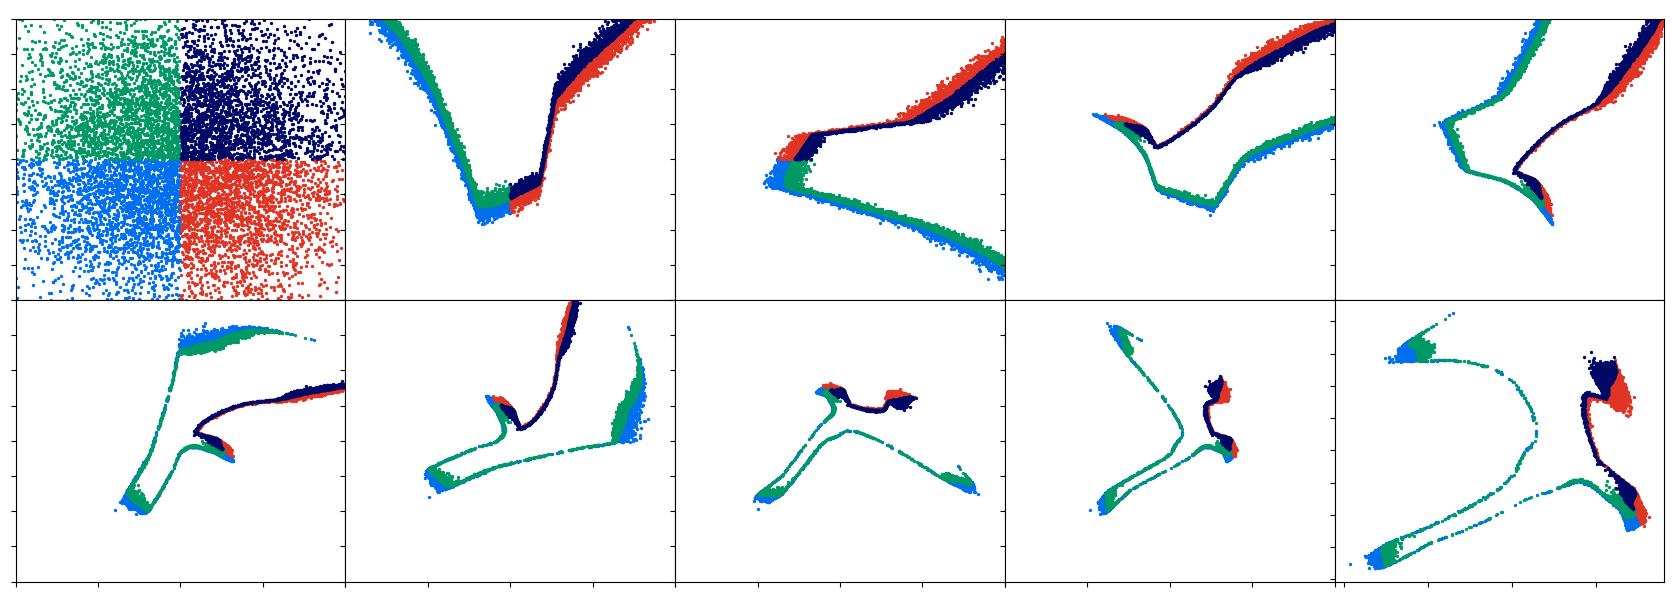
\includegraphics[width=\textwidth]{figures/himmelblau_flow.png}
            \column{0.45\textwidth}
            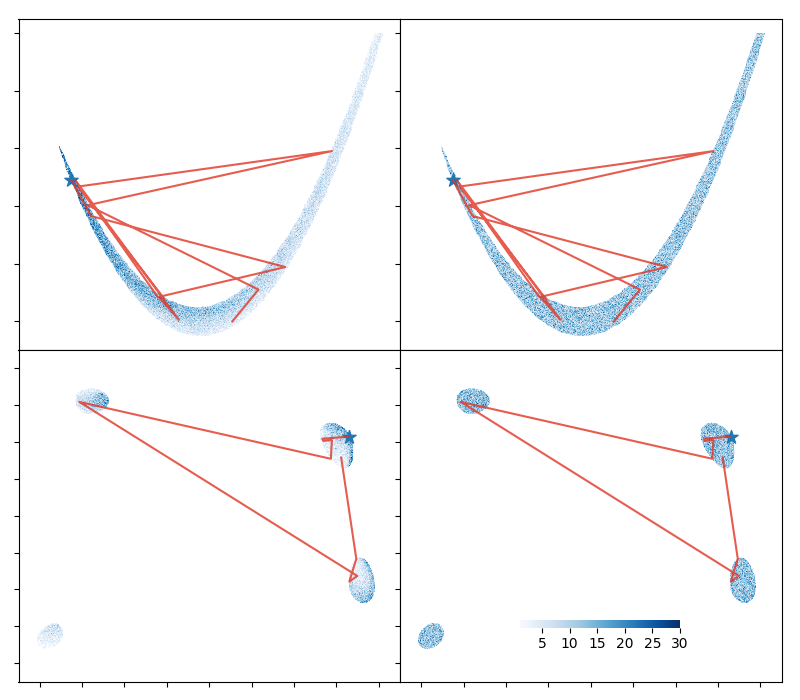
\includegraphics[width=\textwidth]{figures/chains.png}
        \end{columns}
        \texttt{nessai}~\arxiv{2102.11056} \texttt{nora}~\arxiv{2305.19267} \texttt{jaxnest}~\arxiv{2012.15286}
        \vfill
        \column{0.3\textwidth}
        \texttt{DNest}~\arxiv{1606.03757}
        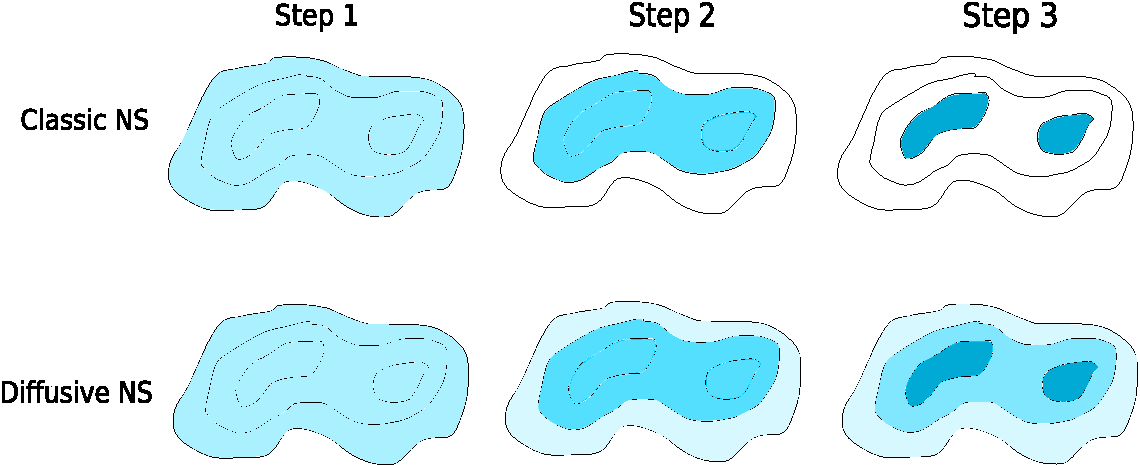
\includegraphics[width=\textwidth]{figures/dnest}
        \texttt{ProxNest}~\arxiv{2106.03646}
        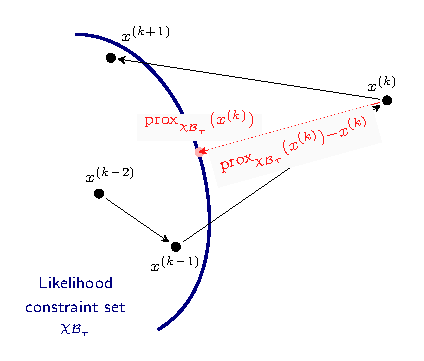
\includegraphics[width=\textwidth]{figures/proxnest_diagram}
        \texttt{dynesty}~\arxiv{1904.02180} 
        \vfill
    \end{columns}
\end{frame}

\begin{frame}
    \frametitle{The nested sampling meta-algorithm: dead points}
    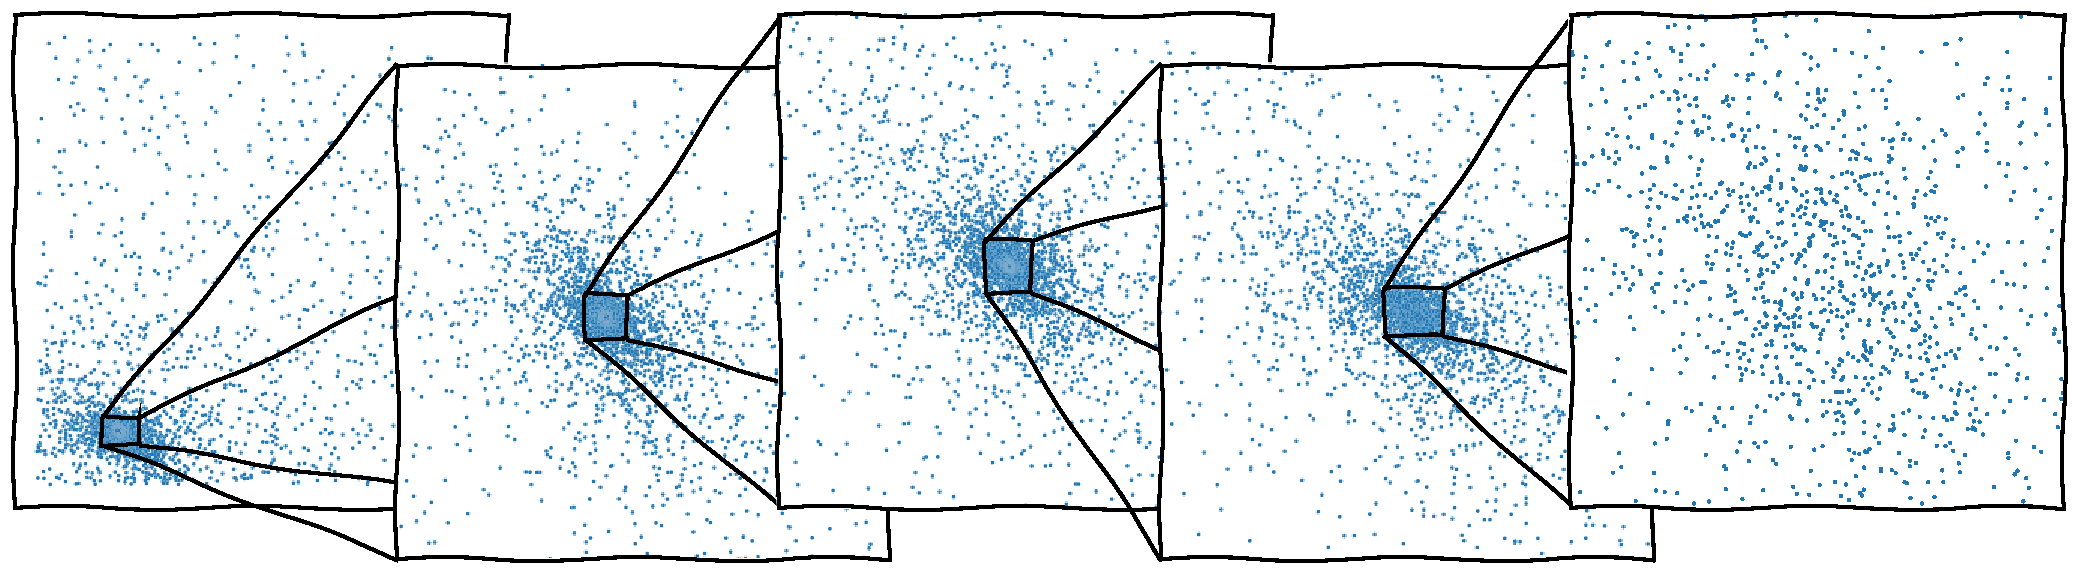
\includegraphics[width=\textwidth]{figures/dead_measure}
    \begin{columns}
        \column{0.69\textwidth}
        \begin{itemize}
            \item At the end, one is left with a set of discarded ``dead'' points.
            \item Dead points have a unique scale-invariant distribution $\propto\: \tfrac{dV}{V}$.
            \item Uniform over original region, exponentially concentrating on region of interest (until termination volume).
            \item Good for training emulators (HERA~\arxiv{2108.07282}).
        \end{itemize}
        \column{0.3\textwidth}
        \begin{block}{Applications}
            \begin{itemize}
                \item training emulators.
                \item gridding simulations
                \item beta flows
                \item ``dead measure'' 
            \end{itemize}
        \end{block}
    \end{columns}
\end{frame}

\begin{frame}
    \frametitle{Similarities}
    \begin{columns}
        \column{0.5\textwidth}
        \includegraphics[width=\textwidth,page=15]{figures/himmelblau}% 
        \column{0.5\textwidth}
        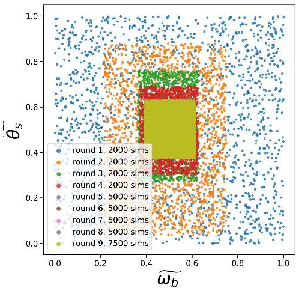
\includegraphics[width=\textwidth]{figures/tmnre.pdf}
    \end{columns}
\end{frame}

\begin{frame}
    \frametitle{Why it's hard to do SBI with nested sampling}
    \begin{itemize}
        \item At each iteration $i$, nested sampling requires you to be able to generate a new live point from the prior, subject to a hard likelihood constraint
            \[ \theta\sim\pi : \mathcal{L}(\theta)>\mathcal{L}_i \]
        \item This is hard if you don't have a likelihood!
        \item In addition, nested sampling does not do well if the likelihood is non-deterministic
        \item Previous attempts:
            \begin{itemize}
                \item DNest paper \arxiv{1606.03757}(Section 10: Nested sampling for ABC)
                \item ANRE~\arxiv{2308.08597} using non-box priors driven by current ratio estimate with slice sampling re-population.
            \end{itemize}
    \end{itemize}
\end{frame}

\begin{frame}
    \frametitle{Sequential NRE with nested sampling}
    \begin{tikzpicture}[
            node distance=1cm,
            >=stealth, auto,
            every state/.style={
                rectangle, rounded corners, minimum width=2em,
                text width=6.8cm, align=center
            }
        ]
        \node[state, fill=C3!20, minimum height=3cm] (q14) {
            \textbf{NS}\\
            Run nested sampling on $\log r_{i}(\theta, D_\text{obs})$ \\
            to generate $\theta$ dead samples between prior and posterior targeted at $D_\text{obs}$.
        };
        \node[state, fill=C0!20, minimum height=1cm] (q121) [above=of q14] {
            \textbf{Terminate} if $\mathcal{D}_\text{KL}$ has converged
        };
        \node[state, fill=C0!20, minimum height=1cm] (q12) [above=of q121] {
            \textbf{Initialise} $\theta\sim\pi$\\
        };
        \node[state, fill=C2!20, minimum height=3cm] (q34) [right=of q14] {
            \textbf{NRE}\\
            Train Neural ratio estimator $\log r_i$
            with weights initialised from previous run
        };
        \node[state, fill=C1!20, minimum height=3cm] (q23) [above=of q34] {
            \textbf{Simulate}\\
            Generate simulations $\theta\to D$ from all discarded points
        };
        \begin{scope}[bend left]%
            \path[thick,-{Latex[width=2mm]}]   (q14.north) edge node {} (q121.south)
            (q121.east) edge node {}($(q23.south west)!0.16!(q23.north west)$) 
            (q23.south) edge node {} (q34.north)
            (q34.west) edge node {} (q14.east)
            (q12.east) edge node {}($(q23.south west)!0.84!(q23.north west)$) ;
        \end{scope}
        \node[align=center] (e) at (barycentric cs:q121=0.5,q12=0.5,q23=1,q34=1,q14=1) {\Large\textbf{NSNRE}};
    \end{tikzpicture}
\end{frame}

\begin{frame}
    \frametitle{\texttt{PolySwyft}}
    \begin{columns}[t]
        \column{0.45\textwidth}
        \begin{block}{\texttt{PolyChord}}
            \tthref{github.com/PolyChord/PolyChordLite}
            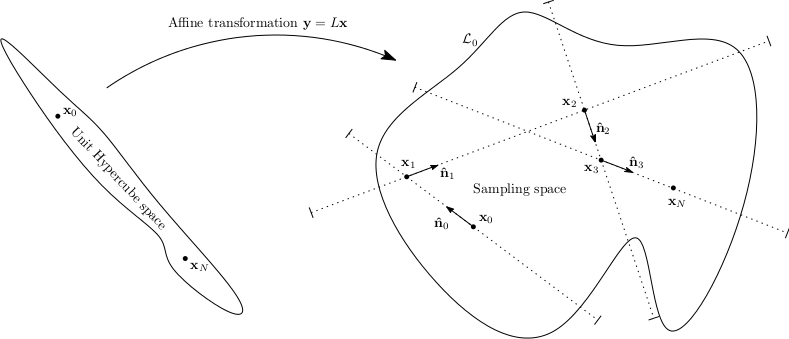
\includegraphics[width=\textwidth]{figures/polychord.png}
            \begin{itemize}
                \item Widely used high-performance nested sampling tool (implementing slice sampling \& clustering in MPI Fortran)
            \end{itemize}
        \end{block}
        \column{0.45\textwidth}
        \begin{block}{\texttt{Swyft}}
            \tthref{github.com/undark-lab/swyft}
            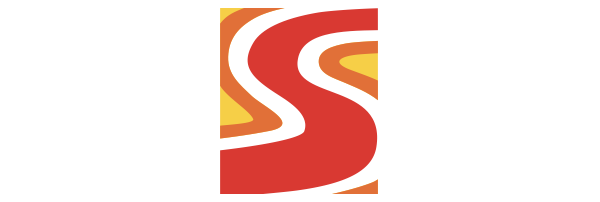
\includegraphics[width=\textwidth]{figures/swyft_logo_wide.png}
            \begin{itemize}
                \item Widely used TMNRE tool in cosmology/astrophysics.
            \end{itemize}
        \end{block}
        However, NSNRE is general, and not specific to these choices.
    \end{columns}
\end{frame}

\begin{frame}
    \frametitle{Convergence diagnostics}
    \begin{columns}
        \column{0.5\textwidth}
        \begin{itemize}
            \item Example for a $n=5$ dimensional parameter space, with $d=100$ data points, (\texttt{lsbi} gaussian mixture model).
            \item This is the regime for cosmological scale problems.
            \item To determine convergence we track:
                \begin{itemize}
                    \item The change in KL divergence between rounds (\C[0]{blue}), and check when this goes to zero.
                    \item The total KL divergence between prior and posterior estimate (\C[1]{orange}), and check when this levels off (ground truth in \C[3]{red}).
                    \item Also shown is the KL divergence between the estimate and the ground truth (\C[2]{green}).
                \end{itemize}
        \end{itemize}
        \column{0.5\textwidth}
        \includegraphics<1>[width=\textwidth]{figures/GMM_posterior_estimates.pdf}%
        \includegraphics<2|handout:0>[width=\textwidth]{figures/GMM_KL_div_per_round.pdf}
    \end{columns}
\end{frame}

\begin{frame}
    \frametitle{Conclusions}
    \framesubtitle{\tthref{github.com/handley-lab}}
    \tikz[overlay,remember picture]
    \node[anchor=north east] (A) at ($(current page.north east)+(0,0)$) {
        
\includegraphics[width=0.09\textheight]{figures/students/adam_ormondroyd.jpg}%
        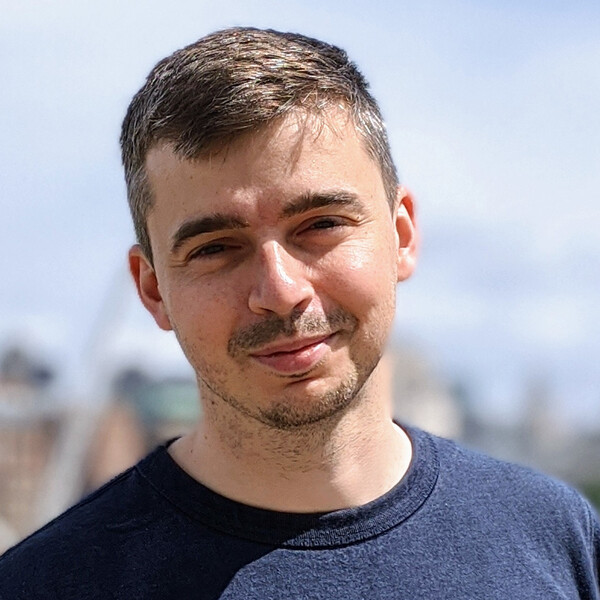
\includegraphics[width=0.09\textheight]{figures/students/david_yallup.jpg}%
        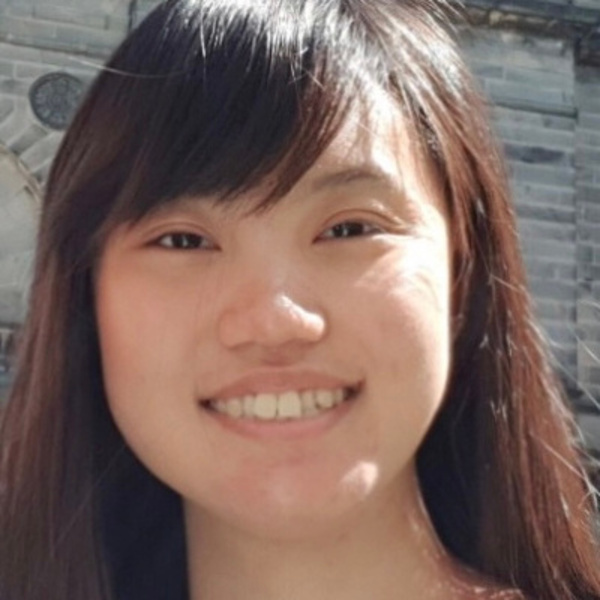
\includegraphics[width=0.09\textheight]{figures/students/dily_ong.jpg}%
        
\includegraphics[width=0.09\textheight]{figures/students/george_carter.jpg}%
        
\includegraphics[width=0.09\textheight]{figures/students/harry_bevins.jpg}%
        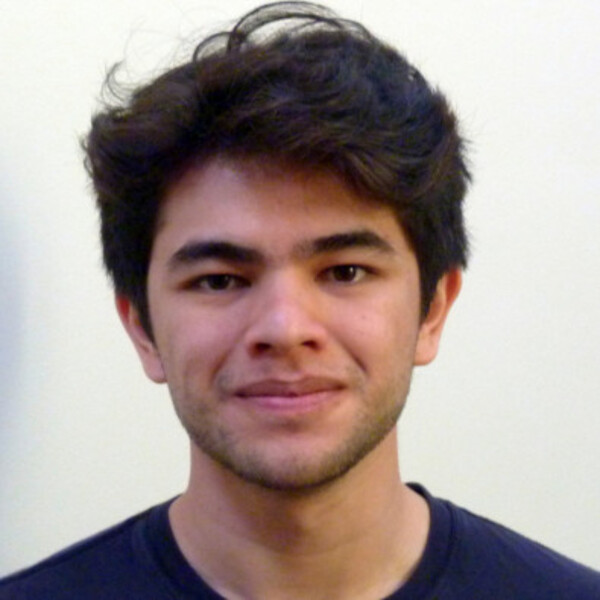
\includegraphics[width=0.09\textheight]{figures/students/ian_roque.jpg}%
        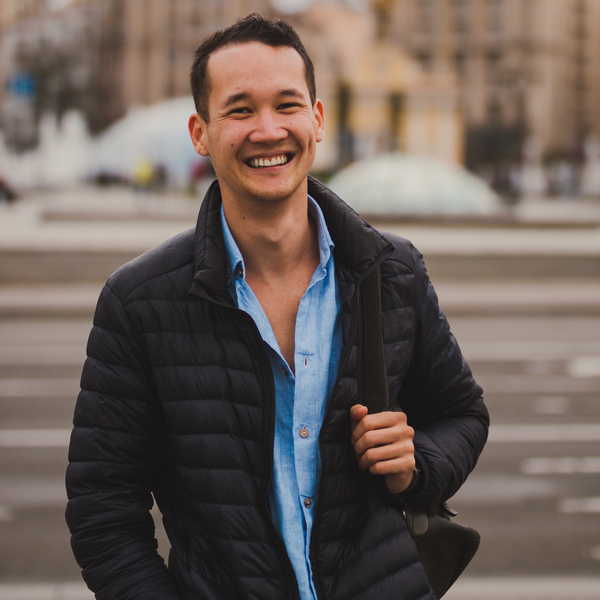
\includegraphics[width=0.09\textheight]{figures/students/kilian_scheutwinkel.jpg}%
        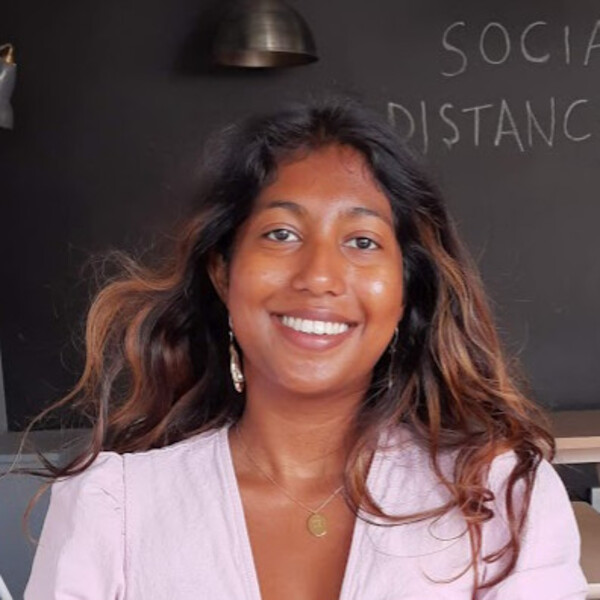
\includegraphics[width=0.09\textheight]{figures/students/metha_prathaban.jpg}%
        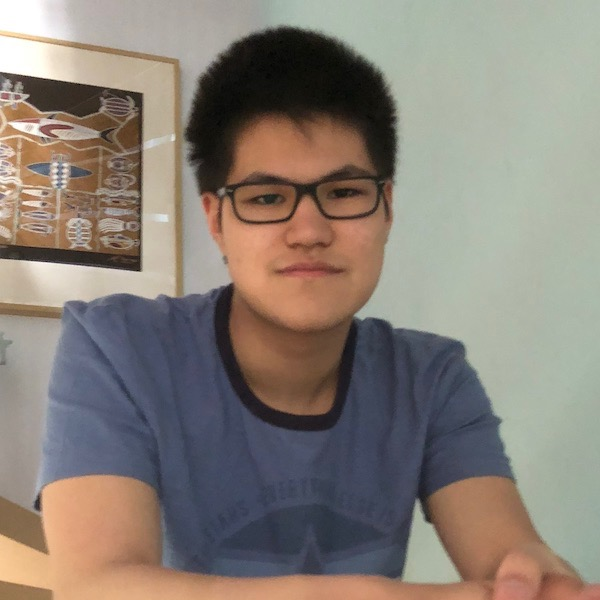
\includegraphics[width=0.09\textheight]{figures/students/namu_kroupa.jpg}%
        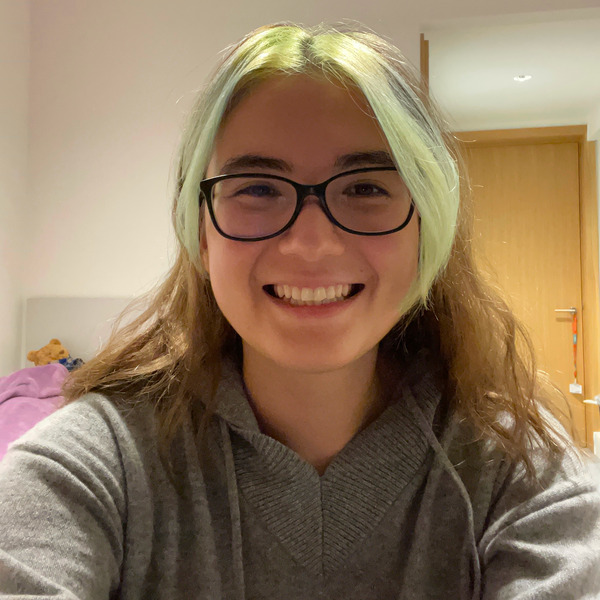
\includegraphics[width=0.09\textheight]{figures/students/sinah_legner.jpg}%
        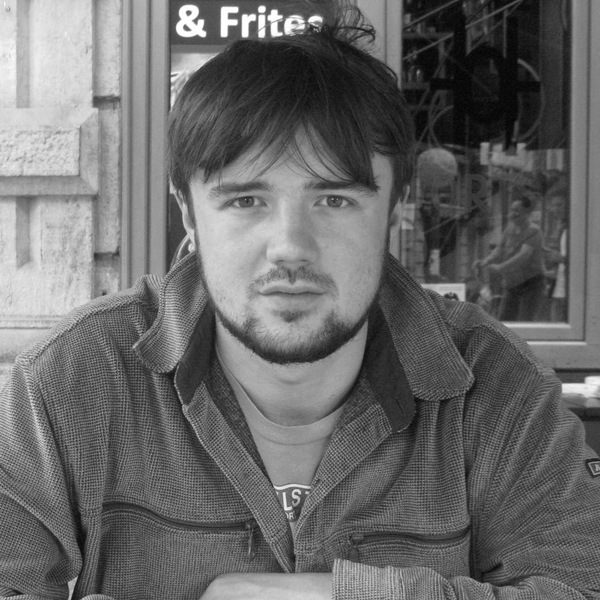
\includegraphics[width=0.09\textheight]{figures/students/sam_leeney.jpg}%
        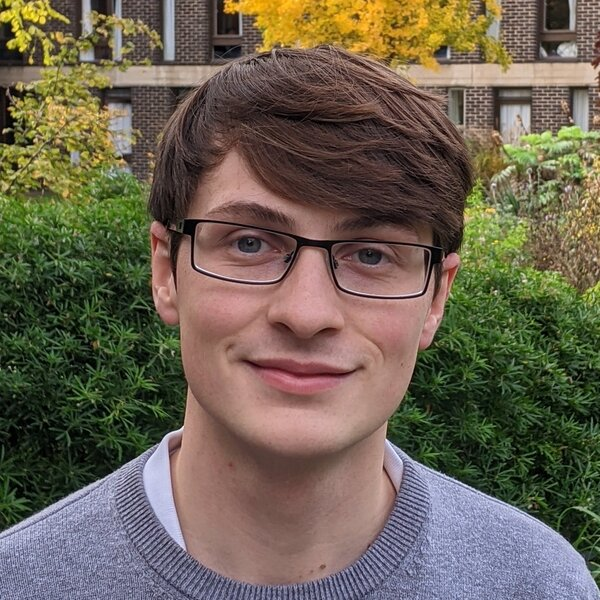
\includegraphics[width=0.09\textheight]{figures/students/thomas_gessey-jones.jpg}%
        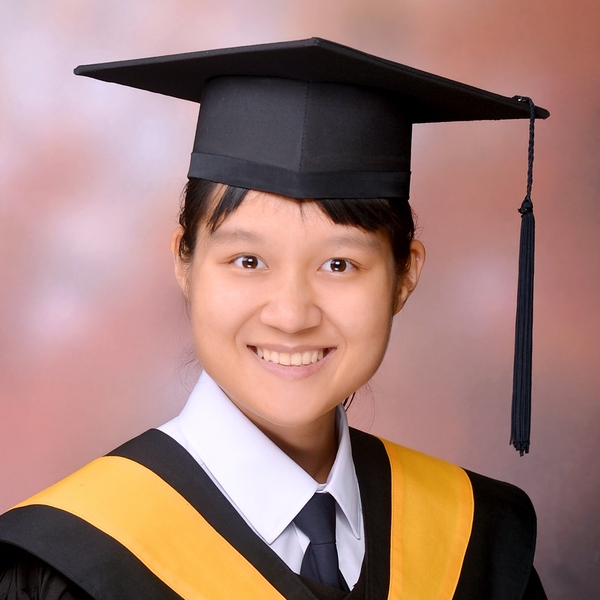
\includegraphics[width=0.09\textheight]{figures/students/wei-ning_deng.jpg}%
    };
    \begin{itemize}
        %\item What does NSNRE give you that TMNRE doesn't?
        %    \begin{itemize}
        %        \item Use of dead points which scan from prior to logr peak avoids risk of 'trimming' important regions of the space
        %        \item Likelihood-driven contours allow more parameters $n>2$ to be considered in comparison with box priors
        %    \end{itemize}
        \item \texttt{PolySwyft} can perform NRE on $n\sim 6$ parameter spaces and $d\sim100$ data spaces.
        \item This makes it relevant for cosmological applications.
        \item Look out for imminent paper (post Kilian's thesis hand-in in $\sim\mathcal{O}(1 \text{month}))$
        %\item Investigating this raises (?existential) questions regarding NRE.
        %\item Is the $-5 <\log r < 5$ saturation of NREs a fundamental problem, or an engineering one?
        %\item Is there a ``nested'' approach to crossing this range in larger parameter spaces $n\gg 5$?
        \item Examples produced using \texttt{lsbi} package: \tthref{github.com/handley-lab/lsbi}\\
    \end{itemize}
\end{frame}

\appendix

\begin{frame}
    \frametitle{Considerations of ratio estimation}
    \student{zixiao_hu}{Zixiao Hu}{MPhil}
    \begin{columns}
        \column{0.5\textwidth}
        \begin{itemize}
            \item Neural REs can in practice only estimate in a band of $\log r$ before the activation function saturates (typically $-5 < \log r < 5$).
            \item Consider a posterior $\mathcal{P}$ well approximated by a Gaussian profile in an $n$-dimensional parameter space~\arxiv{2312.00294}
            \item If $\mathcal{D}_\text{KL}\gg1$ between prior and posterior:
                \begin{gather*}
                    \log r = \frac{n}{2} + \mathcal{D}_\text{KL} + \chi^2_{n} \\
            %\[\mathcal{P}(\log r) = \frac{1}{\Gamma(\tfrac{n}{2})} e^{\log r-\frac{n}{2}-\mathcal{D}_\text{KL}} \left(\tfrac{n}{2}+\mathcal{D}_\text{KL}-\log r\right)^{\frac{n}{2}-1}\]
            %i.e. $\log r$ has an offset \& rescaled chi-squared distribution:
            %\[n + 2\mathcal{D}_\text{KL} - 2\log r \sim \chi^2_{n} \]
                    \left\langle \log r \right\rangle_\mathcal{P} = \mathcal{D}_\text{KL}, \qquad \sigma(\log r)_\mathcal{P} = \sqrt{\frac{n}{2}}
                \end{gather*}
            \item Truncation ({\bf T}MNRE) reduces $\mathcal{D}_\text{KL}$, focusing the distribution into the $[-5,5]$ band.
            \item Marginalisation (T{\bf M}NRE) reduces $n$ \& $\sigma$.
        \end{itemize}
        \column{0.5\textwidth}
        \vspace{10pt}
        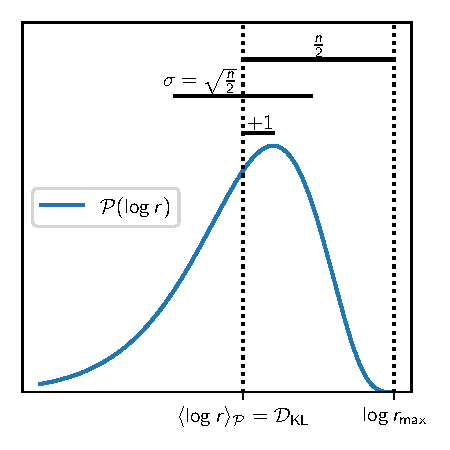
\includegraphics{figures/anatomy}
    \end{columns}
\end{frame}

\begin{frame}
    \frametitle{Cosmological forecasting}
    \framesubtitle{Have you ever done a Fisher forecast, and then felt Bayesian guilt?}
    \vspace{-20pt}
    \begin{columns}[t]
        \column{0.5\textwidth}
        \begin{itemize}
            \item Cosmologists are interested in forecasting what a Bayesian analysis of future data might produce.
            \item Useful for:
                \begin{itemize}
                    \item white papers/grants,
                    \item optimising existing instruments/strategies,
                    \item picking theory/observation to explore next.
                \end{itemize}
            \item To do this properly:
                \begin{enumerate}
                    \item start from current knowledge $\pi(\theta)$, derived from current data
                    \item Pick potential dataset $D$ that might be collected from $P(D)\: (=\mathcal{Z})$
                    \item Derive posterior $P(\theta|D)$
                    \item Summarise science (e.g. constraint on $\theta$, ability to perform model comparison)
                \end{enumerate}
        \end{itemize}
        \column{0.5\textwidth}
        \begin{itemize}
            \item This procedure should be marginalised over:
                \begin{enumerate}
                    \item All possible parameters $\theta$ (consistent with prior knowledge)
                    \item All possible data $D$
                \end{enumerate}
            \item i.e. marginalised over the joint $P(\theta,D)=P(D|\theta)P(\theta)$.
            \item Historically this has proven very challenging.
            \item Most analyses assume a fiducial cosmology $\theta_*$, and/or a Gaussian likelihood/posterior (c.f. Fisher forecasting).
            \item This runs the risk of biasing forecasts by baking in a given theory/data realisation.
        \end{itemize}
    \end{columns}
\end{frame}

\begin{frame}
    \frametitle{Fully Bayesian Forecasting~\arxiv{2309.06942}}
    \student{thomas_gessey-jones}{Thomas Gessey-Jones}{PhD}
    \begin{columns}
        \column{0.5\textwidth}
        \begin{itemize}
            \item Simulation based inference gives us the language to marginalise over parameters $\theta$ and possible future data $D$.
            \item Evidence networks give us the ability to do this at scale for forecasting~\arxiv{2305.11241}.
            \item Demonstrated in 21cm global experiments, marginalising over:
                \begin{itemize}
                    \item theoretical uncertainty
                    \item foreground uncertainty
                    \item systematic uncertainty
                \end{itemize}
            \item Able to say ``at 67mK radiometer noise'', have a 50\% chance of 5$\sigma$ Bayes factor detection.
            \item Can use to optimise instrument design
            \item Re-usable package: \texttt{prescience}
        \end{itemize}
        \column{0.5\textwidth}
        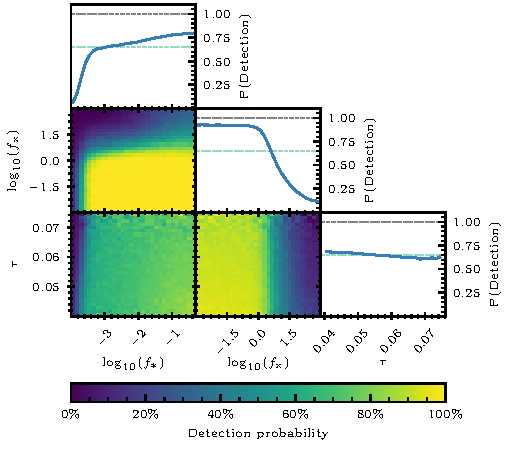
\includegraphics[width=\textwidth]{figures/fbf.pdf}
    \end{columns}
\end{frame}

\end{document}
